\documentclass[11pt,letterpaper]{article}

\usepackage{setspace}
%\doublespacing
\linespread{1.25}
%\linespread{2}
\usepackage{geometry}

\geometry{letterpaper, margin=1in}
%\usepackage{times}
\usepackage{pslatex}
\usepackage{apacite}
\usepackage{url}
\usepackage{graphicx}
\usepackage{caption}
\usepackage{subcaption}
\usepackage{listings}
\usepackage{color}
\usepackage{textcomp}
\usepackage{amsmath}
\usepackage{amssymb}
\usepackage{wrapfig}
\usepackage{lipsum}

\graphicspath{{figures/}}

\def\signed #1{{\leavevmode\unskip\nobreak\hfil\penalty50\hskip2em
  \hbox{}\nobreak\hfil(#1)%
  \parfillskip=0pt \finalhyphendemerits=0 \endgraf}}

\newsavebox\mybox
\newenvironment{aquote}[1]
  {\savebox\mybox{#1}\begin{quote}}
  {\signed{\usebox\mybox}\end{quote}}


 \newcommand{\denote}[1]{\mbox{ $[\![ #1 ]\!]$}}

\definecolor{Red}{RGB}{255,0,0}
\newcommand{\red}[1]{\textcolor{Red}{#1}}  
\definecolor{Green}{RGB}{10,200,100}
\definecolor{Blue}{RGB}{10,100,200}
\newcommand{\ndg}[1]{\textcolor{Green}{[ndg: #1]}}  
\newcommand{\mht}[1]{\textcolor{Blue}{[mht: #1]}}  

\usepackage{titlesec}

\setcounter{secnumdepth}{4}

\titleformat{\paragraph}
{\normalfont\normalsize\bfseries}{\theparagraph}{1em}{}
\titlespacing*{\paragraph}
{0pt}{3.25ex plus 1ex minus .2ex}{1.5ex plus .2ex}

\title{Talking in generalizations}
%\author{{\large \bf Michael Henry Tessler} and {\large \bf Noah D. Goodman} \\
%\{mtessler, ngoodman\} @stanford.edu\\
%  Department of Psychology, Stanford University}

\begin{document}

\maketitle

Learning and development require solving problems of induction.
To understand that swans are white, one must generalize the property \textsc{is white} to the category of swans.
Similarly, events can be generalized and made useful for future predictions of behavior and outcomes (e.g. Bill smokes cigarettes, Smoking causes cancer). 
Observation and pedagogy are available methods early on in development for solving these inductive problems \cite{Markman1989, Shafto2012}.
Around the age of two, generalizations get conveyed with language \cite{Cimpian2008, Gelman2008}. 
%Adults and young children overcome this hard problem by merely observing instances of the category \cite{Markman1989} and potentially more robustly by being shown the same evidence pedagogically \cite<e.g.>{Shafto2012}.
%More to the point, a helpful interlocutor could just tell you \emph{Swans are white}. 

\emph{Generic} language is a simple and convenient way to communicate generalization about categories (e.g.~\emph{Swans are white}), and similar linguistic devices are available for generalizations about events (habituals, e.g. \emph{Bill smokes cigarettes}) and causes (causals, e.g. \emph{Smoking causes cancer}; \citeNP{Carlson1977, Carlson2005, Cohen1999, Leslie2008}). 
%Similar, simple sentences are used to communication generalizations about events, called \emph{habituals} (e.g.  Bill smoking a cigarette can be generalized over time with ; \citeNP{}). 
%Even statements about causality can be thought of as generalizing a particular cause--effect instance (e.g. Bill getting cancer as a result of smoking) over time and space  (e.g. \emph{Smoking causes cancer}).
%and generalizations about causes---\emph{causals}generalizes over the instances where smoking was the cause of a cancer).
%Similarly, it is useful to generalize particular events (e.g. \textsc{bill smoking a cigarette}) over time (e.g. \textsc{bill smokes cigarettes}), and generalize a cause that occurred in a particular place at a particular time (e.g. \textsc{bill's cancer was caused by smoking}) to a causal relationship that occurs invariant of space and time (e.g. \textsc{smoking causes cancer}).
%Making such generalizations is tricky though can be achieved by adults and young children by learning from evidence
%and, particularly so, in pedagogically enriched contexts \cite{Markman1989, Shafto2012}.
%The task is made almost trivial, though, if the generalization is communicated with language (e.g. somebody tells you: \emph{Swans are white.}).
%At about age of the two, a new tool for communication and learning becomes available: language.
%Generalizations can be made about the properties of a category (e.g. \emph{Dogs are friendly}),
%events that tend to occur 
%and about causal relationships that tend to hold 
%Generalizations may also be conveyed with language.
%Generic (e.g.~\emph{Swans are white}), habitual (e.g.~\emph{Bill smokes cigarettes}), and causal (e.g.~\emph{Smoking causes cancer}) language provide common and simple ways to communicate generalizations. 
%We take category generalizations as our primary case study, extend our analysis to habitual language later, and speculate on causal language at the end. 
%Generic language is ubiquitous in everyday conversation and in child-directed speech \cite{Gelman2008} and children as young as two or three understand that generics refer to categories and support generalization \cite{Cimpian2008}.
Learning through generic statements, in particular, is essential to the growth of conceptual knowledge \cite{Gelman2004} and how kinds are represented in the mind \cite{Leslie2008}.
%Similar processes may be occurring for habitual language with respect to drawing inferences about stable properties of individuals \cite{Gelman1999}.
Despite the apparent simplicity of the language and their centrality to learning, a formal account of generic meaning remains elusive. 

The primary hurdle in formalizing generic language is in determining what makes a generic sentence true or false (i.e. the truth conditions).
%Generics look a lot like quantifier statements (e.g. \emph{some, all, most}).
At first blush, generics look a lot like universally quantified statements as in \emph{All swans are white}, and yet generics---unlike universals---admit exceptions (e.g. there are black swans). 
Interpreting the generic as meaning ``most'' (i.e. \emph{Most swans are white}) captures many cases but fails to account for others: \emph{Robins lay eggs} seems true even though only adult, female robins do; only a tiny fraction of Mosquitos carry the virus Zika yet \emph{Mosquitos carry Zika} also sounds true. 
In fact, the very notion that the felicity of the generic can be tied to how many instances have the property (in the way that quantifier statements are) violates intuitions: \emph{Robins lay eggs} even though only the females do but \emph{Robins are female} is not a reasonable thing to say (even though only the females are).

%Habitual sentences behave in an analogous way. 
%Bill may smoke a pack a day and so we would say \emph{Bill smokes}, and if Bill goes without a cigarette for an entire family vacation (thus temporarily reducing his effective rate of smoking), we will not be so easily convinced (i.e. \emph{Bill smokes} is probably still true).
%Cases like \emph{Mosquitos carry malaria} (wherein only a tiny percentage have the property) seem to parallel habitual sentences of rare actions like \emph{Susan writes novels}. Susan may only have written 3 novels in her life, but still this seems like a valid generalization to convey.

We argue that the core meaning of generic and habitual sentences is simple but underspecified, and that general principles of pragmatic reasoning are responsible for establishing a precise meaning in context. 
Building on recent probabilistic models of language understanding, we provide a formal model for the evaluation of generic sentences, which in principle generalize to other generalizations conveyed in language (e.g. habituals, causals). 
This model explains the puzzling flexibility in truth conditions (e.g. \emph{Birds lay eggs} vs. \emph{Birds are female}; \emph{Mosquitos carry Zika}) in terms of diverse prior beliefs about properties.
In Experiment 1, we elicit these priors experimentally and show that the resulting model predictions explain almost all of the variance in human truth judgments for familiar generic sentences.
Experiment 2 demonstrates that the same model accounts for truth judgments for a wide range of habitual sentences, where frequency alone would fail.
Finally, using habitual language, we show in Experiment 3 that communicating generalizations is sensitive to top-down moderators of expectations: It is the subjective belief of future behavior (not just what has been observed objectively in the past) that matters for communicating generalizations.
%Generalizations about categories, however, are just one kind of generalization.
%Habitual sentences describe generalizations about events (e.g. \emph{Bill smokes}, \emph{Susan mows her neighbor's lawn.}; \citeNP{Carlson1977, Carlson2005, Cohen1999}). 


\subsubsection*{A formal model of generic meaning}

Generics express a relation between a kind (e.g. \textsc{robins}) and a property (e.g. \textsc{lays eggs}). 
For a given kind $K$ (e.g.~\textsc{robins}) and property $F$ (e.g.~\textsc{lays eggs}), we refer to the probability that an object of kind $K$ has property $F$, that is $P(F\mid K)$, as the \emph{prevalence} of $F$ within $K$.
\footnote{Because we aim to explain the psycholinguistics of generics, we are generally interested in the subjective probability, not the actual frequency in the world.}
Logical quantifiers can be described as conditions on prevalence (i.e.~\emph{some} is $P(F\mid K)>0$, \emph{all} is $P(F\mid K)=1$). 
Extending this, it seems the simplest meaning for generic statements would be a similar threshold on prevalence: $P(F\mid K)>\tau$ \cite{Cohen1999}. 
However, no fixed value of the threshold, $\tau$, would allow for the extreme flexibility generics exhibit (e.g. \emph{Robins lay eggs} vs. \emph{Robins are female}; \emph{Mosquitos carry Zika}).
Building on \citeA{Lassiter2013,Lassiter2015}, we posit that this threshold is not a fixed property of the language, but is established by pragmatic inference.

Using the Rational Speech-Acts framework \cite{Frank2012,Goodman2013}, 
we model a speaker $S_2$ who reasons about a pragmatic listener $L_1$; this listener is considering the prevalence of a certain property within the category.
The listener $L_1$ doesn't know the appropriate threshold for the generic in this context ($\tau \sim \text{Uniform}$(0,1)), and reasons about what an informative speaker $S_1$ would be likely to say. The hypothetical speaker $S_1$ in turn reasons about an idealized literal listener $L_0$, who has access to the threshold $\tau$ (i.e. $S_1$ believes $L_0$ will interpret him in exactly the way he means). 
Writing the prevalence as $x$, this leads to a set of equations:
%
\begin{eqnarray}
P_{S_{2}}(u \mid x) & \propto &  \int_{\tau} P_{L_{1}}(x , \tau \mid u) \label{eq:S2}\\
P_{L_{1}}(x , \tau \mid u) &\propto& P_{S_{1}}(u \mid x, \tau) \cdot P(x) \cdot P(\tau) \label{eq:L1}\\
P_{S_{1}}(u \mid x, \tau) &\propto&  {P_{L_{0}}(x \mid u, \tau)}^{\alpha} \label{eq:S1}\\
P_{L_{0}}(x \mid u, \tau) &\propto& {\delta_{\denote{u}(x, \tau)} P(x)}. \label{eq:L0}
\end{eqnarray}
%
We take the pragmatic speaker $S_2$ to consider two utterances: the generic, with $\denote{u}(x, \tau) := x>\tau$, or nothing (staying silent), with $\denote{u}(x, \tau) := \text{True}$.
Equation \ref{eq:S2} can then be interpreted as a model of felicity or truth judgments \cite{Degen2014}.
The speaker will choose to produce the generic when the true prevalence $x$ is more likely under $L_1$'s posterior given the generic than under her prior (implied by $S_2$ ``staying silent''). 
A fully implemented version of the model can be found at \url{http://forestdb.org/models/generics.html}.

Generalizations about events (e.g.~\emph{Bill smokes}) are modeled by specifying the underlying scale to be the rate with which an event occurs (e.g. Bill smokes cigarettes 4 times a day.) rather than the prevalence of the property. 
The rest of the model is the same.



%We measured it empirically (n=60) for a set of properties (e.g. \textsc{lays eggs, carries malaria}; 21 in total) used in our target sentences. 
 


\subsubsection*{Summary of experiments and results}

\begin{figure}[t]
\centering
  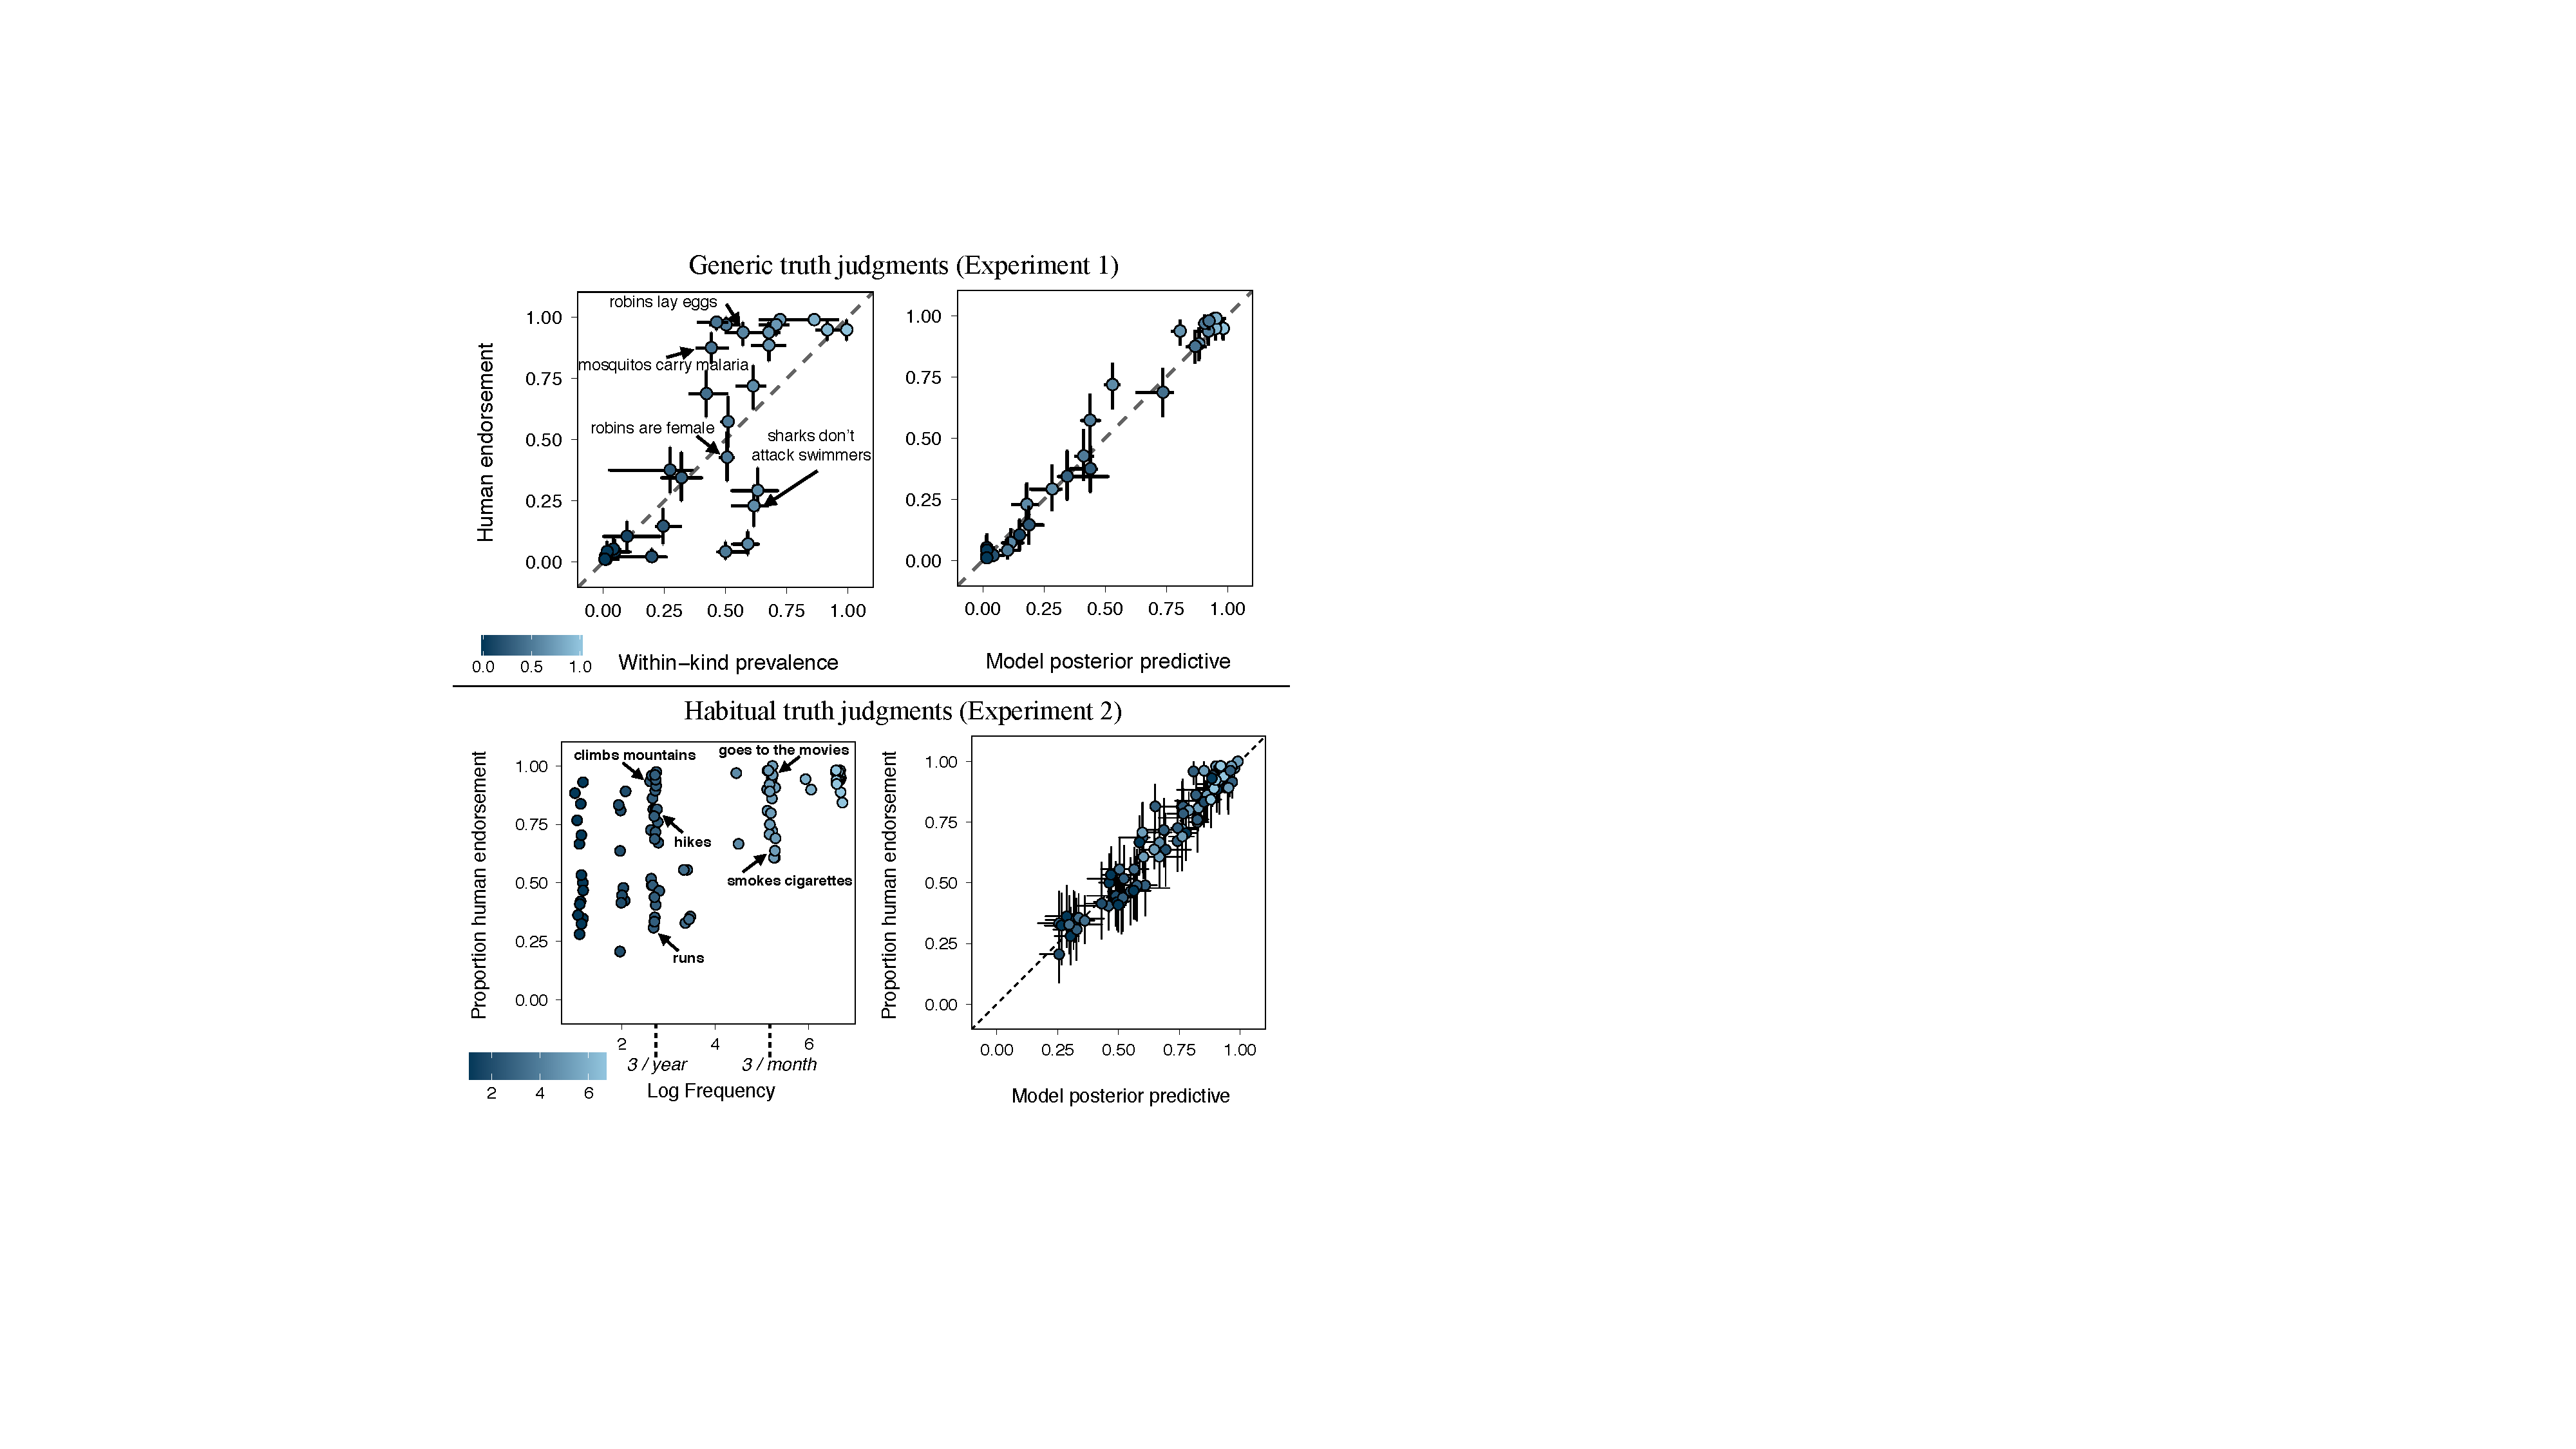
\includegraphics[width=0.75\textwidth]{tj-2x2}
  \caption{Human acceptability judgments for generic (top) and habitual (bottom) sentences vs. Left: the prevalence of the property measured in Expt.~1 (e.g.~50\% of robins are female) and log frequency of action given to the participant in Expt.~2 (e.g. Last month, Bill smoked cigarettes 3 times), and 
  Right: speaker $S_2$ (Eq.~\ref{eq:S2}) model predictions.
%  and speaker $S_2$ model predictions (right) for ninety-three unique items (event \textsc{x} frequency). 
  Color denotes target-category prevalence and target-individual frequency of action, with lighter colors indicating more prevalent properties and more frequent actions. 
%  Actual frequency noted on x-axis for examples (left).
  Error bars correspond to 95\% bootstrapped confidence intervals for the human data and 95\% Bayesian credible intervals for the model predictions. 
  Error bars suppressed and points jittered on bottom, left facet for visual clarity.}
  \label{fig:tj}
\end{figure}


In three experiments, we test the felicity of various generic and habitual sentences, and compare the speaker model in Eq.~\ref{eq:S2} to the human truth judgments. 
Experiment 1 ($n=100$) uses generic sentences of familiar categories (e.g.~\emph{Birds lay eggs}; \emph{Birds are female}) with no further information present.
Experiment 2 ($n=150$) uses habitual sentences of novel characters (e.g.~\emph{Bill smokes cigarettes}) and presents information about the frequency with which the event has occurred in the past (e.g. Last week, Bill smoked cigarettes 3 times.). 
For both of the experiments, we measure empirically the prior distribution $P(x)$ over prevalence ($n=60$) or propensity ($n=40$), respectively.
%In both Experiment 1 and Experiment 2, we use the empirically elicited priors and the speaker $S_2$ model to predict the truth judgments of generic and habitual sentences, respectively. 
In both cases, the speaker $S_2$ model explains almost all of the variance in human endorsements of generic and habitual sentences ($r^2(30) = 0.98$ and $r^2(93) = 0.94$, respectively) while using just the prevalence \emph{within} the particular category or just the rate of the event explains relatively little of the data ($r^2(30) = 0.59$ and $r^2(93) = 0.33$; Figure \ref{fig:tj}).

In Experiment 3, we present participants with the same stimuli as in Expt.~2 and include extra information that either enables (e.g. Yesterday, Bill bought a pack of cigarettes.) or disables (e.g. Yesterday, Bill decided to quit smoking) the event from occurring. 
We measure participants' predictions ($n=120$) about the future frequency with which the target person will do the action (e.g. ``In the next week, how many times will Bill smoke cigarettes?'') and a set of different participants ($n=150$) rated the felicity of the habitual sentence. 
The speaker model $S_2$ who attempts to communicate the past frequency explains almost none of the data $r^2(63)=0.02$ while the model that wants to communicate the future frequency explains much of the data $r^2(63)=0.91$.
We also find that when no additional information is present, predicted frequency perfectly tracks past frequency (and so the two models have the same predictions for the data in Expt.~2).

In sum, our model that decides if a generic sentence is a pragmatically useful way to describe a category (or if a habitual is a useful way to describe an individual's behavior) by taking into account the listener's prior beliefs about the property (or event)---how common it is and the likely prevalence or frequency (measured empirically)---explains the puzzling flexibility of truth conditions for generic and habitual language.
This work provides a formal bridge between our intuitive theories of categories and events, and the words we use to describe them.
%We validated this model by eliciting felicity judgments for generic and habitual sentences covering diverse properties and activities (Expt.~1b, 2b).
%To our knowledge, the experiments presented here are first empirical investigations into the truth conditions of habitual sentences and the first test of a formal model of habitual language.

%However, the enabling and disabling conditions 



%The prior $P(x)$ describes the belief distribution on the prevalence of a given property (e.g. \textsc{lays eggs}) across relevant categories for the case of generic sentences and on the rate of a given event (e.g. \textsc{smoking}) across individuals for the case of habitual sentences. 
%The shape of this distribution affects model predictions, but may vary significantly among different properties.
%We measure it empirically for a diverse set of properties ($n=40$ for use in Expt.~1) and for a set of events ($n=40$ for use in Expts.~2\&3).


%\subsubsection*{Method}
%
%We recruited 60 participants over Amazon's crowd-sourcing platform Mechanical Turk (MTurk).  
%%We chose this number of participants based on intuition with similar experiments and model comparison; 
%%since this is a quantitative experiment with no planned comparisons, power analysis in not appropriate.
%Participants were restricted to those with US IP addresses and with at least a 95\% MTurk work approval rating (the same criteria apply to all experiments reported). 
%
%On each trial of the experiment, participants filled out a table where each row was an animal category and each column was a property. 
%In order to alleviate the dependence of the distribution on our animal categories of interest, half of the animal categories were self-generated by the participant; the other half were randomly sampled from a set corresponding to the generic sentences used in Expt. 1b (e.g. \textsc{robins, mosquitos}).
%Participants were asked to fill in each row with the percentage of members of each of the species that had the property (e.g. ``50\%'').
%Each participant reported on sixteen properties (see {\it SI Section A} for more details).
%We used a set of properties associated with generics of theoretical interest (twenty-one properties in total), as described above.
% 
%\subsubsection*{Data analysis and results}
 
%\subsubsection*{Discussion}



%Yet the meaning of generic language is philosophically puzzling and has resisted precise formalization.
%We explore the idea that the core meaning of a generic sentence is simple but underspecified, 
%and that general principles of pragmatic reasoning are responsible for establishing the precise meaning in context.
%Building on recent probabilistic models of language understanding, we provide a formal model for the evaluation and comprehension of generic sentences. 
%This theory provides the mathematical bridge between the words we use and the concepts they describe.


\bibliographystyle{apacite}

\setlength{\bibleftmargin}{.125in}
\setlength{\bibindent}{-\bibleftmargin}

\bibliography{generics-spp}

\end{document}

